% !TEX encoding = UTF-8 Unicode

\documentclass[a4paper]{article}

\usepackage{color}
\usepackage{url}
\usepackage[utf8]{inputenc} % make weird characters work
\usepackage{graphicx}
\usepackage[english,serbian]{babel}
\usepackage[unicode]{hyperref}
\usepackage{amsthm}
\usepackage{amssymb}
\hypersetup{colorlinks,citecolor=green,filecolor=green,linkcolor=blue,urlcolor=blue}
\usepackage[title]{appendix}
\usepackage{float}
\usepackage[graphicx]{realboxes}
\usepackage[font=small,labelfont=bf]{caption}
\usepackage{chngcntr}
\counterwithin{figure}{section}
\usepackage{listings}
\definecolor{codegreen}{rgb}{0,0.6,0}
\definecolor{codegray}{rgb}{0.5,0.5,0.5}
\definecolor{codeblue}{rgb}{0.0,0,0.82}
\lstdefinestyle{mystyle}{
    numbers=left,
    numberstyle=\scriptsize,
    numbersep=8pt,
    commentstyle=\color{codegray},
    keywordstyle=\color{codegreen},
    numberstyle=\tiny\color{codeblue},
    stringstyle=\color{codegreen},
    basicstyle=\ttfamily\footnotesize,
    breakatwhitespace=false,
    breaklines=true,
    captionpos=b,
    keepspaces=true,
    showspaces=false,
    showstringspaces=false,
    showtabs=false,
    tabsize=4,
    xleftmargin=3em,
    framexleftmargin=1.5em
}
\lstset{style=mystyle}


\begin{document}

\title{Analiza ``Million Songs'' skupa podataka\\ \small{Seminarski rad u okviru kursa\\Istra\v{z}ivanje podataka\\ Matematički fakultet}}

\author{\href{mailto:mi14042@matf.bg.ac.rs}{Milana Kova\v{c}evi\'c}\\ \href{mailto:ivan_ristovic@math.rs}{Ivan Ristovi\'c}}
\date{jun 2018.}

\maketitle

\abstract{
U ovom radu su dati rezultati istra\v{z}ivanja skupa podataka \emph{Million Songs Dataset}. Nakon kratkog opisa strukture samog skupa, opisan je na\v{c}in na koji je on obradjen kako bi se prilagodio kori\v{s}\'c{}enim alatima. Uo\v{c}ene su zna\v{c}ajne zavisnosti izmedju atributa. Neke od ovih informacija su dobijene vizuelizacijom skupa atributa, dok su druge dobijene kao izlazi odredjenih algoritama. Postupak analize podataka je detaljno opisan, a najbolje rezultate analize je dao algoritam \emph{Apriori}.
}


\tableofcontents

\newpage

\section{Opis skupa podataka}
\label{sec:Opis skupa podataka}

\emph{The Million Song Dataset} \cite{Dataset} je skup od milion slogova koji sadr\v{z}e informacije o popularnim pesmama. S obzirom da ovaj skup preveliki za udoban rad, ograni\v{c}i\'c{}emo se na podskup od deset hiljada slogova izdvojen od strane autora originalnog skupa.

Svaki slog pomenutog skupa podataka sadr\v{z}i informacije o jednoj pesmi: detalje o izvodja\v{c}u, segmentima, tempu kao i ID pesme na raznim online servisima (\emph{Echo Nest} \cite{EchoNest}, \emph{7digital} \cite{7digital},  \emph{MusicBrainz} \cite{MusicBrainz} i \emph{PlayMe} \cite{PlayMe}). Detaljne informacije o atributima se mogu videti na slici \ref{fig:Atributi}. Primer jednog sloga se mo\v{z}e videti u dodatku \ref{sec:DodatakPrimer}.

Skup u svojoj originalnoj formi je organizovan u \emph{HDF5} format \cite{HDF5}. Mi \'c{}emo izdvojiti informacije iz datog modela i podatke organizovati u CSV format, zarad lak\v{s}eg ubacivanja u alate koje \'c{}emo opisati kasnije. Ova transformacija je izvr\v{s}ena kori\v{s}\'c{}enjem Python skripti iz MSongsDB repozitorijuma \cite{MSongsDB}, modifikovanih za na\v{s}e potrebe. Kompletne skripte se mogu na\'c{}i u dodatku \ref{sec:DodatakIzvlacenje}.

\section{Kori\v{s}\'c{}eni alati}
\label{sec:Alati}

Za obradu podataka, kori\'s{}\'c{}eni su alati \emph{Knime Analytics Platform} \cite{KNIME} i \emph{IBM SPSS Modeler} \cite{SPSS}. \emph{IBM SPSS Modeler} je prete\v{z}no kori\v{s}\'c{}en za vizuelizaciju, dok je \emph{KNIME AP} kori\'s{}\'c{}en za manipulisanje podacima, vizuelizaciju i primenu algoritama. Jupyter svesku \cite{jupyter} smo koristili za dodatnu vizuelizaciju podataka.

\section{Preprocesiranje i vizualizacija podataka}
\label{sec:Preprocesiranje}

U ovom odeljku \'c{}emo poku\v{s}ati da \v{c}itaoca upoznamo sa skupom podataka. Uz vizualne prikaze raznovrsnosti skupa i analize njegovih specifi\v{c}nosti do\v{s}li smo do bitnih zaklju\v{c}aka koji su kasnije uticali na dalje istra\v{z}ivanje skupa i njegovih karakteristika.

Pre samog preprocesiranja podataka koje je neophodno za istra\v{z}ivanje, izvr\v{s}ili smo analizu statisti\v{c}kih podataka dobijenih na osnovu skupa. Dobijene statistike se mogu videti u dodatku \ref{sec:Statistika}.

Neki od atributa koji su vizuelizovani kasnije u ovom odeljku nisu u potpunosti prisutni u skupu, tako da je analiza takvih atributa radjena samo nad slogovima gde nema nedostaju\'c{}ih vrednosti za te atribute.

Jedna od op\v{s}tih transformacija je nad atributom koji sadr\v{z}i informacije o \v{z}anru. \v{Z}anr je podatak koji je originalno dat kao niz niski. Medjutim, sadr\v{z}aj ovog niza nije ta\v{c}no definisan, ve\'c{} on ponekad u sebi sadr\v{z}i \v{c}itavu re\v{c}enicu koja opisuje \v{z}anr. Jednostavna, a neophodna transformacija je bila da iz ovog niza izbacimo pojavljivanje re\v{c}i \emph{and}, \v{c}ije je \v{c}esto pojavljivanje remetilo rezultate.

\begin{figure}[H]
    \footnotesize
    \begin{tabular}{|c|c|c|}
        \hline
        Atribut & Tip podatka & Kratki opis \\
        \hline
        analysis sample rate & float & u\v{c}estalost uzorkovanja \\
        artist 7digitalid & int & \emph{7digital} ID izvodja\v{c}a ili -1 \\
        artist familiarity & float & algoritamska aproksimacija \\
        artist hotttnesss & float & algoritamska aproksimacija \\
        artist id & string & \emph{Echo Nest} ID izvodja\v{c}a \\
        artist latitude & float & geografska \v{s}irina \\
        artist location & string & lokacija autora \\
        artist longitude & float & geografska du\v{z}ina \\
        artist mbid & string & MusicBrainz ID izvodja\v{c}a \\
        artist mbtags & array string & niz MusicBrainz tagova \\
        artist mbtags count & array int & broj MusicBrainz tagova \\
        artist name & string & ime autora \\
        artist playmeid & int & \emph{PlayMe} ID izvodja\v{c}a ili -1 \\
        artist terms & array string & niz \emph{Echo Nest} tagova \\
        artist terms freq & array float & frekvencije \emph{Echo Nest} tagova \\
        artist terms weight & array float & te\v{z}ina \emph{Echo Nest} tagova \\
        audio md5 & string & MD5 he\v{s} kod audio zapisa \\
        bars confidence & array float & pouzdanost takta \\
        bars start & array float & niz po\v{c}etaka taktova \\
        beats confidence & array float &pouzdanost ritma \\
        beats start & array float & niz po\v{c}etaka ritmova \\
        danceability & float & algoritamska aproksimacija \\
        duration & float & trajanje audio zapisa (u sekundama) \\
        end of fade in & float & vreme u odnosu na pocetak u kom prestaje\\
        & & fade-in efekat (u sekundama) \\
        energy & float & algoritamska aproksimacija energije \\
        & & pesme od strane slu\v{s}aoca \\
        key & int & tonalitet u kojem je audio zapis \\
        key confidence & float & pouzdanost tonaliteta \\
        loudness & float & prose\v{c}na ja\v{c}ina (u dB) \\
        mode & int & mod - dur ili mol \\
        mode confidence & float & pouzdanost moda \\
        release & string & ime albuma \\
        release 7digitalid & int & \emph{7digital} ID albuma ili -1 \\
        sections confidence & array float & niz pouzdanosti stihova \\
        sections start & array float & po\v{c}eci stihova \\
        segments confidence & array float & niz pouzdanosti segmenata \\
        segments loudness max & array float & nig maksimalnih ja\v{c}ina unutar \\
        & & segmenata (u dB) \\
        segments loudness max time & array float & niz vremena dostizanja maksimalne ja\v{c}ine \\
        & & unutar segmenata \\
        segments loudness max start & array float & niz ja\v{c}ina na po\v{c}ecima segmenata \\
        segments pitches & 2D array float & niz ja\v{c}ina po segmentima, jedna \\
        & & vrednost za svaku notu \\
        segments start & array float & po\v{c}eci segmenata \\
        segments timbre & 2D array float & informacije o teksturi $(MFCC+PCA)$ \\
        similar artists & array string & niz \emph{Echo Nest} sli\v{c}nih izvodja\v{c}a \\
        song hotttnesss & float & algoritamska aproksimacija \\
        song id & string & \emph{Echo Nest} ID pesme \\
        start of fade out & float & vreme u odnosu na pocetak u kom po\v{c}inje \\
        & & fade-out efekat (u sekundama) \\
        tatums confidence & array float & pouzdanost najmanjih elemenata ritma \\
        tatums start & array float & niz najmanjih elemenata ritma \\
        tempo & float & procenjen tempo (u BPM) \\
        time signature & int & procenjen broj ritmova u taktu, npr. 4 \\
        time signature confidence & float & pouzdanost procene broja ritmova u taktu \\
        title & string & naziv pesme \\
        track id & string & \emph{Echo Nest} ID pesme \\
        track 7digitalid & int & ID \emph{7digital} ID pesme ili -1 \\
        year & int & godina izdavanja uzeta sa \emph{MusicBrainz} ili 0 \\
        \hline
    \end{tabular}
    \caption{Svi atributi prisutni u \emph{The Million Song Dataset} skupu podataka}
    \label{fig:Atributi}
\end{figure}


%\section{Vizuelizacija}
%\label{sec:Vizuelizacija}

Vizuelizacija originalnog skupa podataka je prikazana na slici \ref{fig:before}. Nedostaju\'c{}e vrednosti su prikazane belom bojom, dok su plavom bojom predstavljene postoju\'c{}e vrednosti atributa.

\begin{figure}[H]
    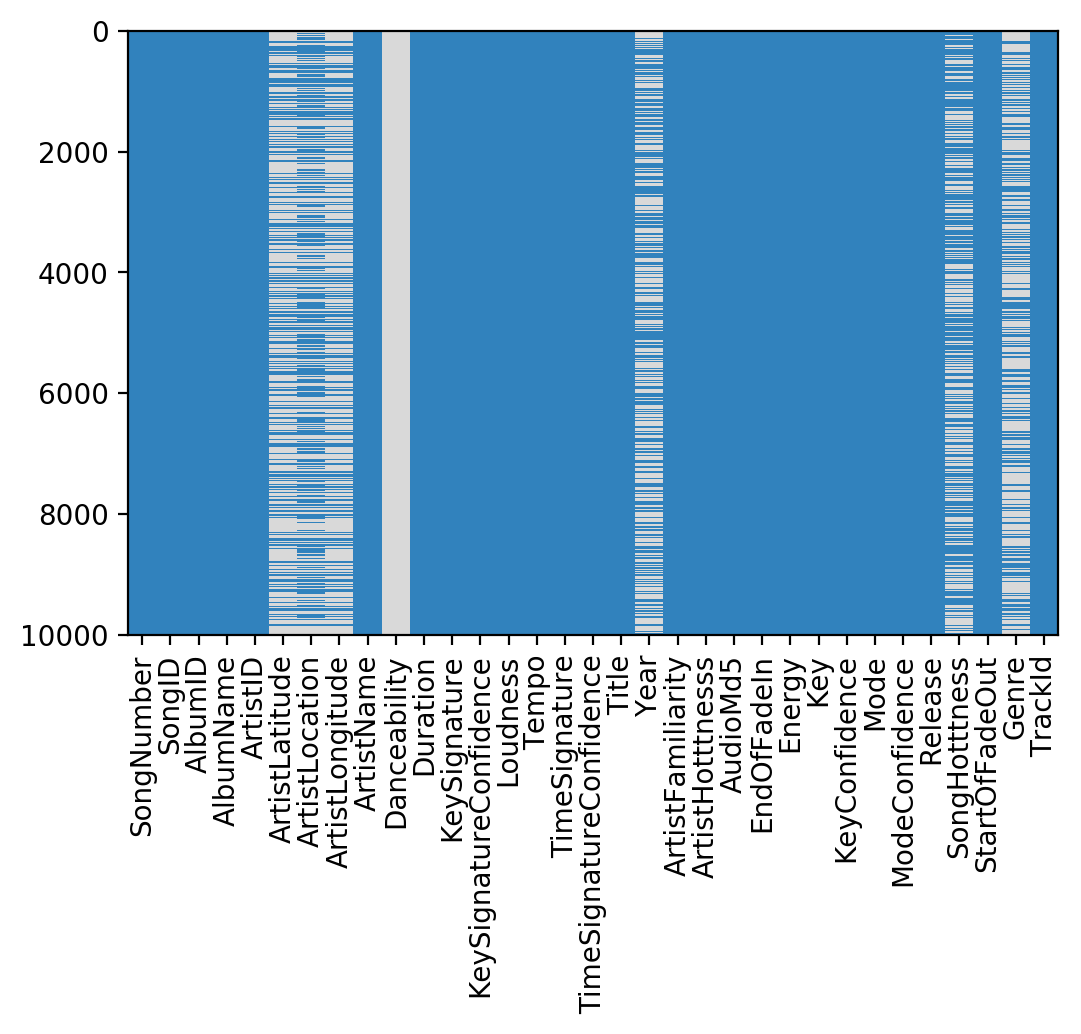
\includegraphics[scale=0.8]{resources/before_processing.png}
    \caption{Nedostaju\'c{}e vrednosti u originalnom skupu podataka}
    \label{fig:before}
\end{figure}

 Sa prikaza skupa podataka se vidi da atribut koji opisuje plesnu mo\'c{} pesme \emph{eng. dancability}, ni u jednom slu\v{c}aju nema postavljenu vrednost, te da je on neupotrebljiv. Takodje, godina, lokacija autora, geografska \v{s}irina, geografska du\v{z}ina i \v{z}anr su atributi koji u velikom broju slu\v{c}ajeva nemaju vrednost. Medjutim, zbog njihove va\v{z}nosti, mi \'c{}emo svoje istra\v{z}ivanje vr\v{s}iti nad onim slogovima za koje su ove vrednosti poznate. Nakon izdvajanja relevantnih atributa za na\v{s}e istra\v{z}ivanje, pripremljen skup podataka je prikazan na slici \ref{fig:after}.

\begin{figure}[H]
    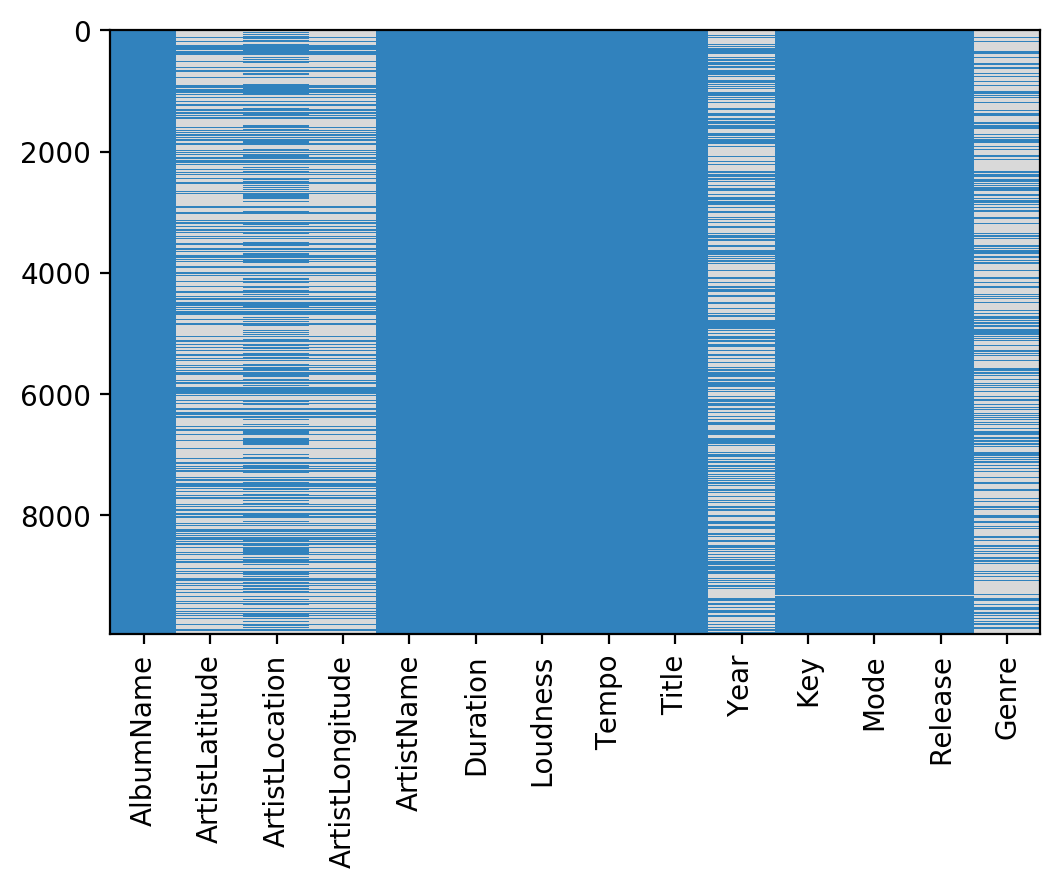
\includegraphics[scale=0.8]{resources/after_processing.png}
    \caption{Izdvojeni atributi kori\v{s}\'c{}eni u istra\v{z}ivanju}
    \label{fig:after}
\end{figure}


Geografska rasprostranjenost autora \v{c}ije su se pesme na\v{s}le u skupu podataka se mo\v{z}e videti na slici \ref{fig:Geolokacija}. Razli\v{c}ite boje predstavljaju vizuelizaciju godine izdavanja pesme - gradijentni prelaz od plave (1950) do crvene (2010).

\begin{figure}[H]
    \centering
    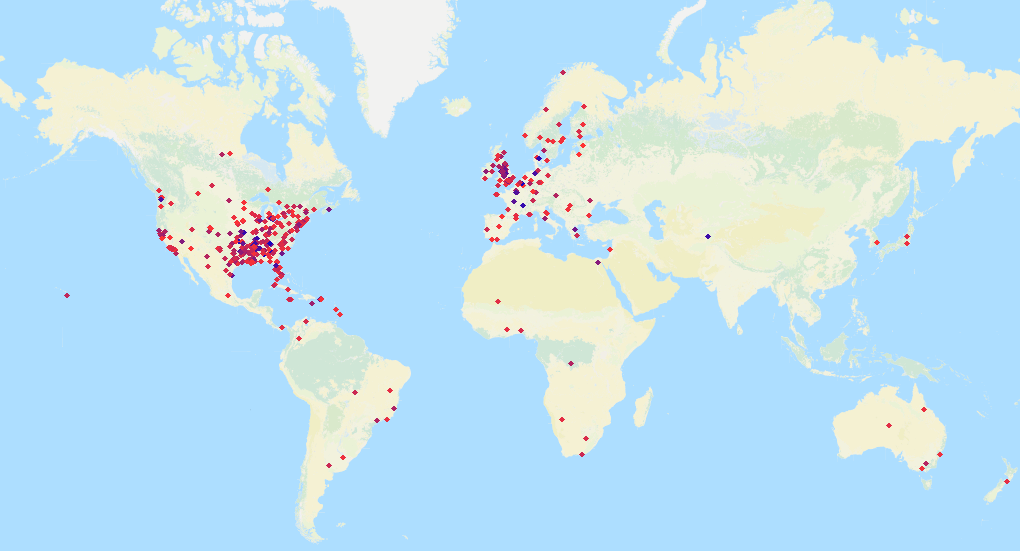
\includegraphics[scale=0.45]{resources/Geolokacija.png}
    \caption{Geografska rasprostranjenost autora}
    \label{fig:Geolokacija}
\end{figure}

Spisak najzastupljenijih zanrova u skupu se mo\v{z}e videti na slici \ref{fig:ZastupljenostZanrova}. \v{Z}anr je atribut sa velikom stopom nedostaju\'c{}ih vrednosti, uz dodatni problem re\v{c}enica prisutnih u nizu (podse\'c{}amo na problem naveden prilikom preprocesiranja, poglavlje \ref{sec:Preprocesiranje}), tako da je analiza vr\v{s}ena nad veoma ograni\v{c}enim skupom od oko tri hiljade slogova. Smatramo, da su ovi rezultati u velikoj meri sli\v{c}ni rezultatima koji bi se dobili da je potpuni skup analiziran - ukoliko ne bi bilo nedostaju\'c{}ih vrednosti za atribut \v{z}anr.

\begin{figure}[H]
    \centering
    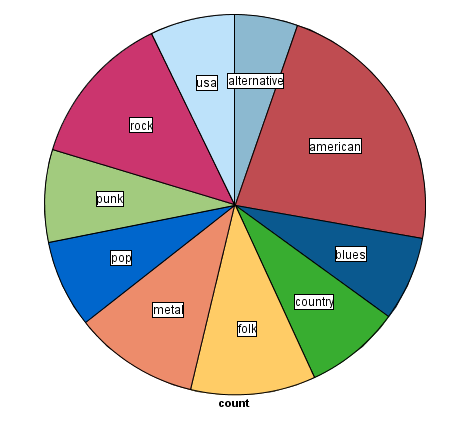
\includegraphics[scale=0.5]{resources/ZastupljenostZanrova.png}
    \caption{Zastupljenost \v{z}anrova}
    \label{fig:ZastupljenostZanrova}
\end{figure}

Vrednosti atributa \emph{duration} prikazane su na grafiku \ref{fig:duration}. Postoji jedna pesma koja ima negativnu du\v{z}inu pa smo najpre izbacili ovu pesmu iz skupa koji obradjujemo. Kako postoje izuzetno duge pesme, nismo postavili gornje ograni\v{c}enje za trajanje pesme.

\begin{figure}[H]
    \centering
    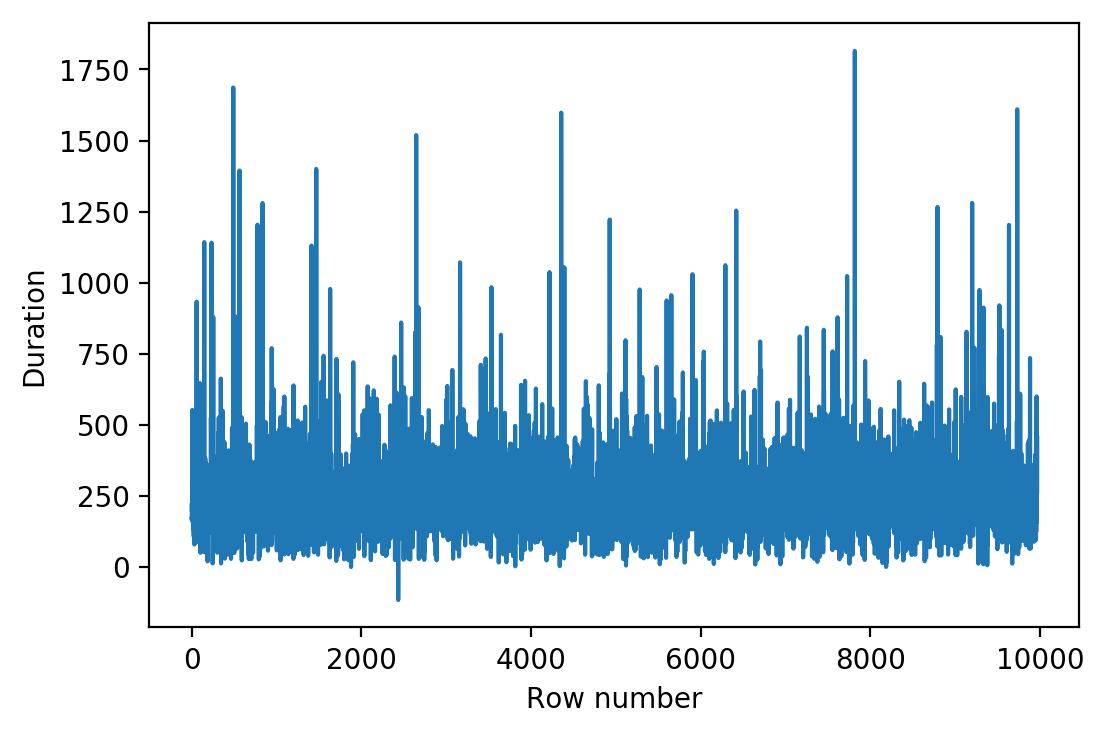
\includegraphics[scale=0.7]{resources/duration.png}
    \caption{Vrednosti atributa \emph{duration}}
    \label{fig:duration}
\end{figure}

Grafik zavisnosti godine i trajanja pesme se mo\v{z}e videti na slici \ref{fig:YearDuration}. Jedan zanimljiv zaklju\v{c}ak koji se name\'c{}e, je da se prose\v{c}no trajanje pesama pove\'c{}ava kroz vreme, sa razlikom od oko 20 sekundi u odnosu na 50-te godine pro\v{s}log veka. Detaljniji prikaz promene proseka trajanja se mo\v{z}e videti na slici \ref{fig:YearDurationAvg}. Takodje, jasno je da se i raznovrsnost pesama mnogo ve\'c{}a danas - prisutne su i veoma kratke ali i veoma duga\v{c}ke pesme.


\begin{figure}[H]
    \centering
    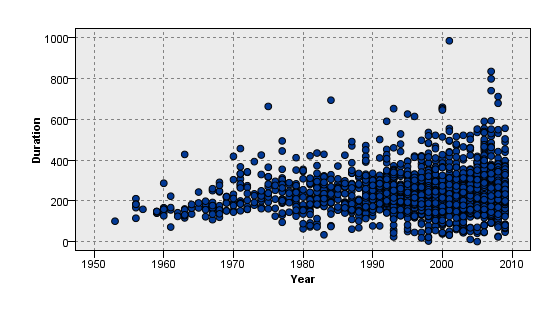
\includegraphics[scale=0.6]{resources/year-duration.png}
    \caption{Odnos godine izdavanja i du\v{z}ine pesme}
    \label{fig:YearDuration}
\end{figure}

\begin{figure}[H]
    \centering
    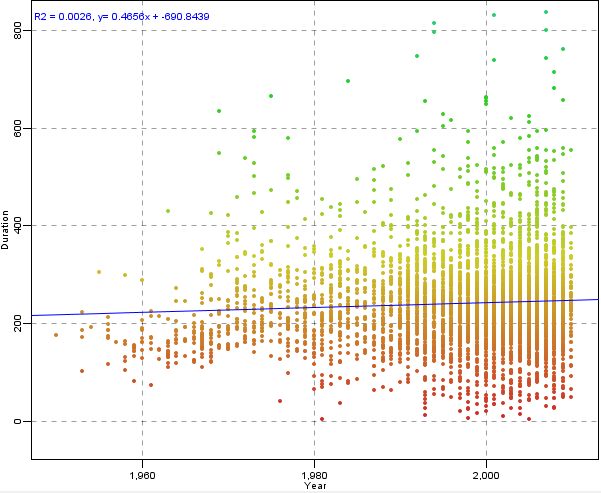
\includegraphics[scale=0.7]{resources/mean-year-duration.PNG}
    \caption{Promena proseka du\v{z}ine pesama kroz vreme}
    \label{fig:YearDurationAvg}
\end{figure}


Prose\v{c}na du\v{z}ina pesama po dr\v{z}avama je prikazana na slici \ref{fig:CountryDuration}. Na\v{z}alost, nisu svi slogovi imali informaciju o nazivu dr\v{z}ave. Iz ovog razloga, dobijenim rezultatima ne treba pridavati veliki zna\v{c}aj.

\begin{figure}[H]
    \centering
    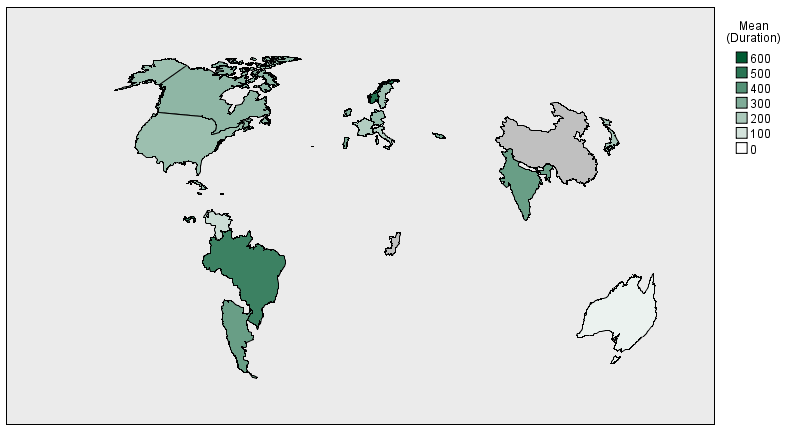
\includegraphics[scale=0.45]{resources/country-duration.png}
    \caption{Prose\v{c}na du\v{z}ina pesama na raznim lokacijama}
    \label{fig:CountryDuration}
\end{figure}


Na slici \ref{fig:loudness} prikazane su vrednosti atributa \emph{loudness}. Ove vrednosti su dobijene na osnovu njihovih proseka tokom trajanja pesme, kao i nekim dodatnim transformacijama. Vise o ovome se mo\v{z}e na\'c{} na zvani\v{c}nom sajtu skupa \cite{Dataset}. Sa grafika se vidi da za atribut \emph{loudness} postoje vrednosti koje izuzetno odstupaju od proseka. Iz toga razloga smo prilikom istra\v{z}ivanja koristili pesme sa vredno\v{s}\'c{}u atributa iz skupa $[-40, 0]$.

\begin{figure}[H]
    \centering
    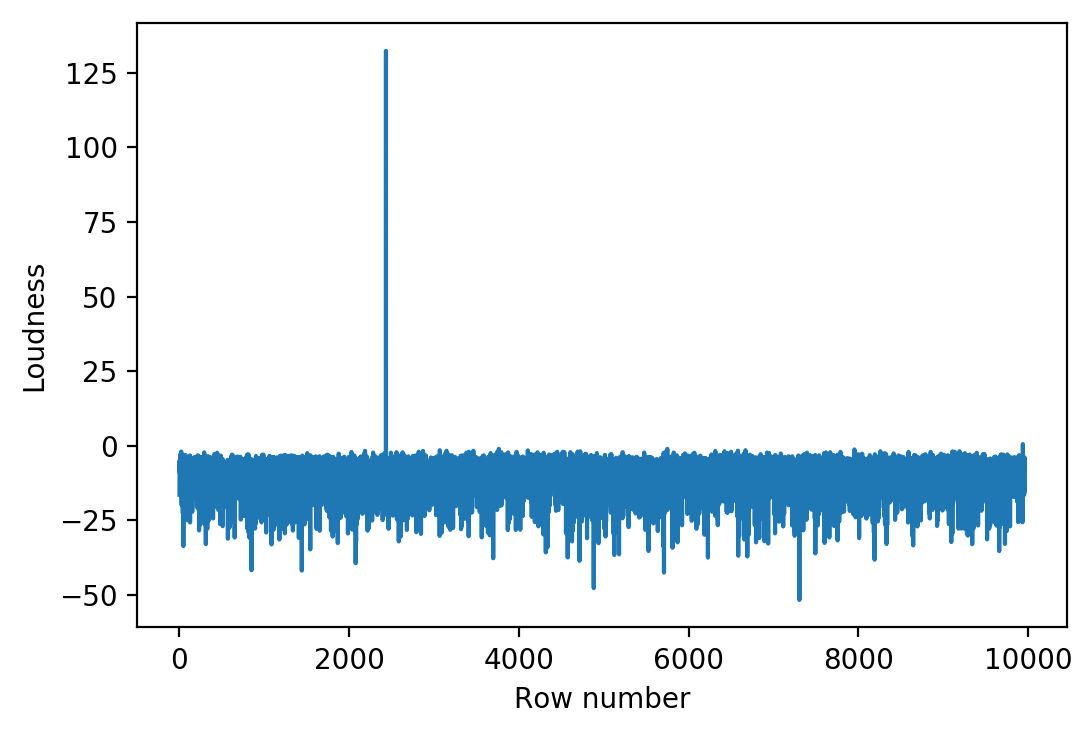
\includegraphics[scale=0.7]{resources/loudness.png}
    \caption{Vrednosti atributa \emph{loudness}}
    \label{fig:loudness}
\end{figure}

Na slici \ref{fig:tempo} prikazane su vrednosti atributa \emph{tempo}. Ovaj atribut sadr\v{z}i nekoliko vrednosti koje su dosta ispod proseka. Medjutim, postoji verovatno\'c{}a da su njima predstvaljene nadprose\v{c}no spore pesme te zbog toga nismo vr\v{s}ili nikakvo odsecanje.

\begin{figure}[H]
    \centering
    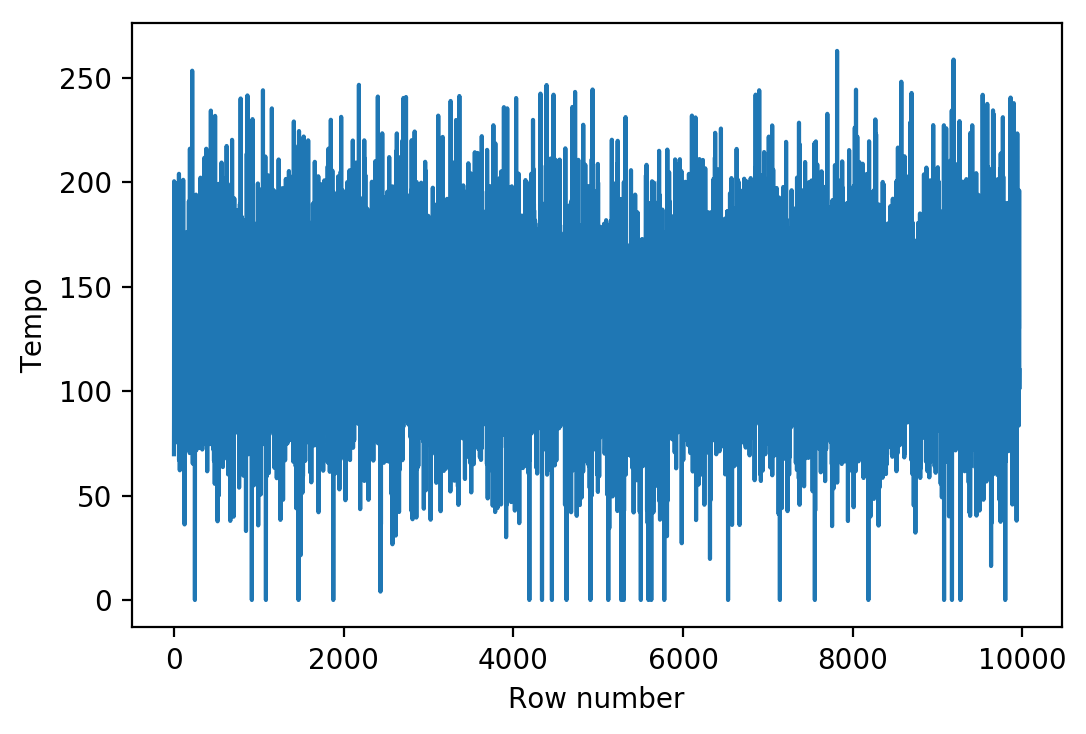
\includegraphics[scale=0.7]{resources/tempo.png}
    \caption{Vrednosti atributa \emph{tempo}}
    \label{fig:tempo}
\end{figure}

S obzirom da \'c{}emo atribute \emph{loudness}, \emph{tempo} i \emph{mode} \footnote{loudness, tempo i mode predstavljaju prose\v{c}nu ja\v{c}inu, tempo i mod (dur ili mol), redom.} koristiti u daljoj analizi (predikcija \v{z}anra pesme) u poglavlju \ref{sec:Klasifikacija}, prikaza\'c{}emo i grafi\v{c}ki prikaz njihove zavisnosti na slici \ref{fig:TempoMode}. Mo\v{z}e se videti da iako pesme oba moda uzimaju raznolike vrednosti za tempo i ja\v{c}inu, mogu\'c{}e je uo\v{c}iti da se pesme sa ekstremnim vrednostima za tempo lep\v{s}e dele po modu. Takodje, mnogo tihe pesme obi\v{c}no pripadaju jednom modu, \v{s}to je i za o\v{c}ekivati jer molske pesme su nekada jako tihe.

\begin{figure}[H]
    \centering
    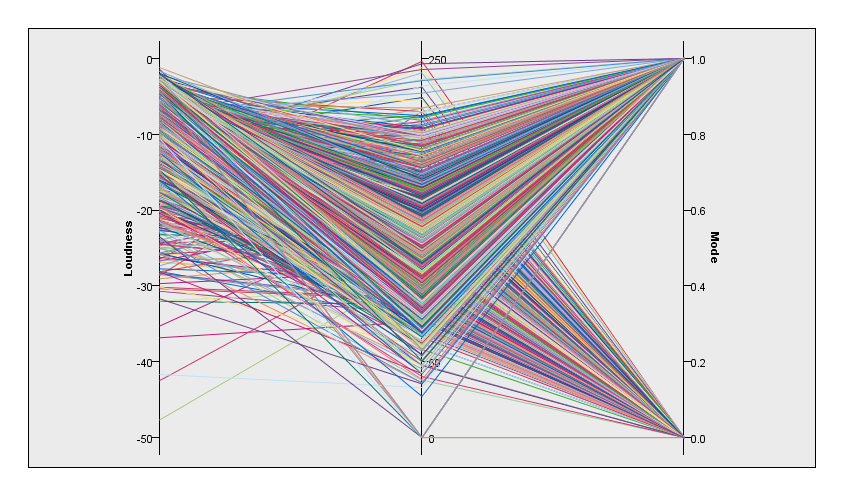
\includegraphics[scale=0.4]{resources/tempo-loudness-mode.png}
    \caption{Prikaz tempa, ja\v{c}ine i moda (dur ili mol)}
    \label{fig:TempoMode}
\end{figure}

\section{Pravila pridru\v{z}ivanja}
\label{sec:PravilaPridruzivanja}

Uo\v{c}avanje zavisnosti izmedju atributa je uradjeno kori\v{s}\'c{}enjem algoritma \emph{Apriori}. Najpre, kao \v{s}to je opisano u poglavlju \ref{sec:Preprocesiranje}, bilo je potrebno eleminisati slogove koji sadr\v{z}e nedostaju\'c{}e vrednosti na relevantnim atributima. Slede\'c{}i korak je zavisio od toga koje su zavisnosti analizirane. Poku\v{s}ali smo da pronadjemo zavisnosti izmedju zanrova, drzava i vremena kreiranja pesme. Rezultati rada Apriori algoritma slede u nastavku. Svi rezultati prikazani ispod su samo deo \v{c}itavog skupa rezultata, izabrani jer smo smatrali da su najinteresantnija.


\subsection{Zavisnosti izmedju \v{z}anrova}
\label{subsec:AprioriZavisnostZanrova}

Nakon prilagodjavanja atributa \emph{\v{z}anr} algoritmu, dobijeni su rezultati prikazani na slici \ref{fig:aprioriZanrovi}. Na njoj je prikazano 10 najizra\v{z}ajnijih pravila sortirana prvo po podr\v{s}ci, a zatim po lift meri, opadaju\'c{}e.
Ovi rezultati su relevantni iako su dobijeni na relativno malim skupom slogova.

\begin{figure}[H]
    \footnotesize
    \centering
    \begin{tabular}{|c|c|c|c|c|}
        \hline
        Podr\v{s}ka & Pouzdanost & Lift mera & Glava pravila & Telo pravila \\
        \hline
        0.2646 & 0.7404 & 1.5567 & rock & pop \\
        0.2646 & 0.5563 & 1.5567 & pop & rock \\
        0.2248 & 0.9930 & 2.0878 & rock & classic \\
        0.2163 & 0.8176 & 3.6114 & classic & pop, rock \\
        0.2163 & 0.9623 & 2.6926 & pop & rock, classic \\
        0.2163 & 1.0000 & 2.1026 & rock & pop, classic \\
        0.1612 & 0.9967 & 2.0957 & rock & indie \\
        0.1405 & 0.9170 & 5.9225 & british & uk \\
        0.1405 & 0.9075 & 5.9225 & uk & british \\
        0.1373 & 0.5582 & 1.1736 & rock & american, classic \\
        \hline
    \end{tabular}
    \caption{Rezultati Apriori algoritma koji pokazuju zavisnost medju \v{z}anrovima}
    \label{fig:aprioriZanrovi}
\end{figure}


\subsection{Zavisnost \v{z}anra od decenije}
\label{subsec:AprioriZavisnostZanraOdDecenije}

Istra\v{z}ivanje koji je \v{z}anr bio zastupljen u nekoj deceniji je dalo no\v{c}ekivane rezultate. Na tabeli \ref{fig:aprioriDecade} prikazana su dobijena pravila zavisnosti sortirana prvo po podr\v{s}ci, a zatim po lift meri, opadaju\'c{}e.
Kako se ranije pokazalo na slici \ref{fig:YearDuration}, najve\'c{}i deo skupa obradjenih podataka pripada dvehiljaditim godinama. Zbog ovoga se dobijeni rezulati koncentri\v{s}u na ovoj deceniji. Kori\v{s}enje ve\'c{}eg i raznovrsnijeg skupa podataka bi doneo druga\v{c}ije rezultate.

\begin{figure}[H]
    \footnotesize
    \centering
    \begin{tabular}{|c|c|c|c|c|}
        \hline
        Podr\v{s}ka & Pouzdanost & Lift mera & Glava pravila & Telo pravila \\
        \hline
        0.0716 & 0.8133 & 1.6369 & 00s & pop, chart \\
        0.0525 & 0.7857 & 1.5815 & 00s & rnb, hop, hall, dance, hip \\
        0.0764 & 0.7385 & 1.4864 & 00s & dance \\
        0.0615 & 0.6824 & 1.3734 & 00s & rnb \\
        0.0615 & 0.6667 & 1.3419 & 00s & hop hip \\
        0.0541 & 0.6000 & 1.2077 & 00s & metal \\
        0.0530 & 0.5917 & 1.1910 & 00s & rock, alternative \\
        0.0578 & 0.5619 & 1.1309 & 00s & alternative \\
        0.0896 & 0.5541 & 1.1153 & 00s & indie \\
        0.0891 & 0.5526 & 1.1123 & 00s & rock, indie \\
        \hline
    \end{tabular}
    \caption{Rezultati Apriori algoritma koji pokazuju zavisnost izmedju \v{z}anrova i decenija tokom koje su bili popularni}
    \label{fig:aprioriDecade}
\end{figure}


\subsection{Zavisnost \v{z}anra od lokacije}
\label{subsec:AprioriZavisnostZanraOdLokacije}

Lokacija autora je atribut \v{c}ije ja vrednost \v{c}esto nepostoju\'c{}a. A ukoliko jeste, iste lokacije su na razli\v{c}itim pesmama druga\v{c}ije napisane. Na primer, jedna pesma ima lokaciju \emph{London}, a druga \emph{London, UK}. Ovakvi podaci su doveli do lo\v{s}ih rezultata istra\v{z}ivanja - slika \ref{fig:aprioriLocation}. Nazalost, jedina pravila koja imaju dovoljno veliku pouzdanost su oblika:
$$\{\emph{uk, british}\} \rightarrow \emph{England}$$
Ovo nam nije od preteranog zna\v{c}aja jer je o\v{c}ekivano da se u Engleskoj slu\v{s}aju pesme \v{z}anra \emph{british}.

\begin{figure}[H]
    \footnotesize
    \centering
    \begin{tabular}{|c|c|c|c|c|}
        \hline
        Podr\v{s}ka & Pouzdanost & Lift mera & Glava pravila & Telo pravila \\
        \hline
        0.0525 & 0.8684 & 7.6535 & England & pop, rock, classic, uk, english, british \\
        0.0541 & 0.7786 & 6.8621 & England & pop, rock, classic, uk, british \\
        0.0546 & 0.8729 & 7.6928 & England & pop, rock, classic, and, english \\
        0.0546 & 0.8729 & 7.6928 & England & rock, classic, uk, english, british \\
        0.0557 & 0.8268 & 7.2865 & England & pop, and, uk, english, british \\
        \hline
    \end{tabular}
    \caption{Rezultati Apriori algoritma koji pokazuju zavisnost izmedju \v{z}anrova i lokacije}
    \label{fig:aprioriLocation}
\end{figure}

\section{Klasterovanje}
\label{sec:Klasterovanje}

Isprobali smo razli\v{c}ite algoritme klasterovanja. Po\v{c}etna ideja je bila da na taj na\v{c}in izdvojimo grupe pesama koje su sli\v{c}ne i prema tome formiramo liste pesama. Ovu ideju smo sproveli algoritmima K-sredina, K-medioida, DBSCAN i algoritmom hijerarhijskog klasterovanja. Medjutim, dobijeni rezultati nisu bili zadovoljavaju\'c{}i te ne\'c{}emo ulaziti u njihovu dublju analizu.

Na slici \ref{fig:knime-klasterovanje} prikazan je KNIME workflow koji smo koristili za isprobavanje algoritama, dok se na slici \ref{fig:kmeans} mogu videti rezultati primene algoritma $k$ sredina.

\begin{figure}[H]
    \centering
    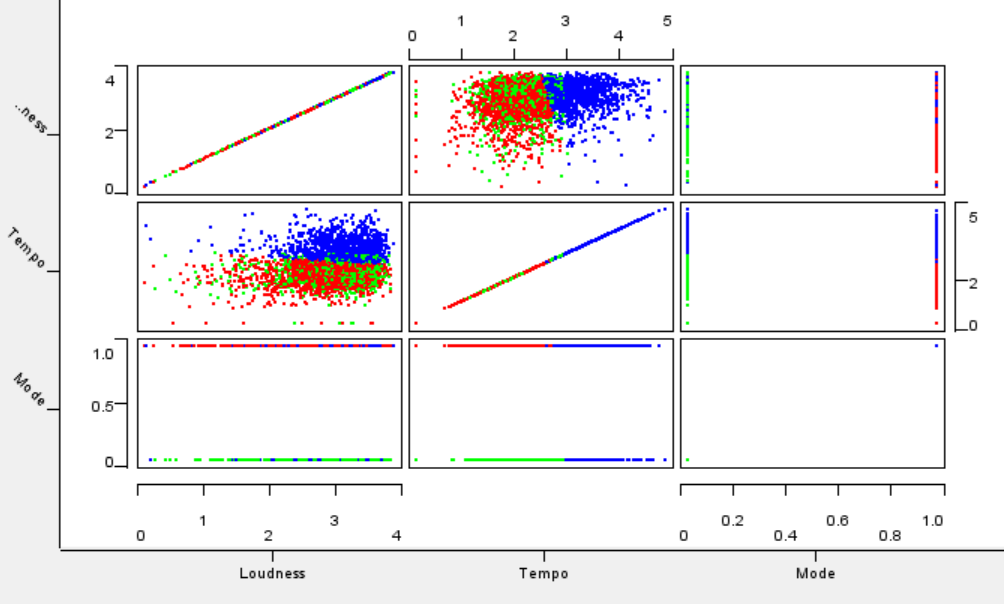
\includegraphics[scale=0.6]{resources/kmeans.png}
    \caption{Rezultat primene algoritma k-means}
    \label{fig:kmeans}
\end{figure}

\begin{figure}[H]
    \centering
    \Rotatebox{90}{%
        \includegraphics[scale=0.7]{KNIME-workflows/screenshots/klasterovanje.PNG}
    }%
    \caption{KNIME workflow za algoritme klasterovanja}
    \label{fig:knime-klasterovanje}
\end{figure}

\section{Klasifikacija}
\label{sec:Klasifikacija}

Jedan od glavnih problema u \v{c}itavom skupu je veliki broj nedostaju\'c{}ih vrednosti za \v{z}anr. Stoga smo poku\v{s}ali da napravimo klasifikator koji \'c{}e klasifikovati instance sa nepoznatim vrednostima za \v{z}anr, treniran nad onim podacima gde su te informacije dostupne.

Prvi problem na koji smo nai\v{s}li su nestandarne vrednosti za \v{z}anr (videti poglavlje \ref{sec:Preprocesiranje}), stoga smo kori\v{s}\'c{}enjem jednostavnih transformacija izvukli slogove sa nedvosmislenom vredno\v{s}\'c{}u za \v{z}anr, a eliminisali one koji su za \v{z}anr imali vrednosti koje nisu bile od zna\v{c}aja za analizu (neki slogovi su imali vi\v{s}e razli\v{c}tih \v{z}anrova). Takodje smo neke sli\v{c}ne \v{z}anrove spojili u jedan, zarad jednostavnijeg rada (na primer \emph{jazz} i \emph{blues} se \v{c}esto pojavljuju zajedno ih ima smisla posmatrati kao jedan \v{z}anr).

Za predikciju vrednosti \v{z}anra smo koristili atribite \emph{loudness}, \emph{tempo} i \emph{mode}. Na\v{z}alost, iz njihove prostorne rasprostranjenosti se vidi da ne postoji jednostavni separator instanci raznih klasa - slika \ref{fig:ZanrKlasifikacija}.

\subsection{Klasifikacija metodom K najbli\v{z}ih suseda}
\label{subsec:knn}

Prva stvar koju smo odlu\v{c}ili da isprobamo bila je \emph{KNN} algoritam u nadi da \'c{}e male grupe pesama istog \v{z}anra lepo klasifikovati bliske instance. O\v{c}ekivano, najbolji model koji smo dobili je imao preciznost od $52.65\%$. Na slici \ref{fig:KNNgreske} se mo\v{z}e videti kako se gre\v{s}ka menjala sa razli\v{c}itim vrednostima za parametar $k$.

\begin{figure}[H]
    \centering
    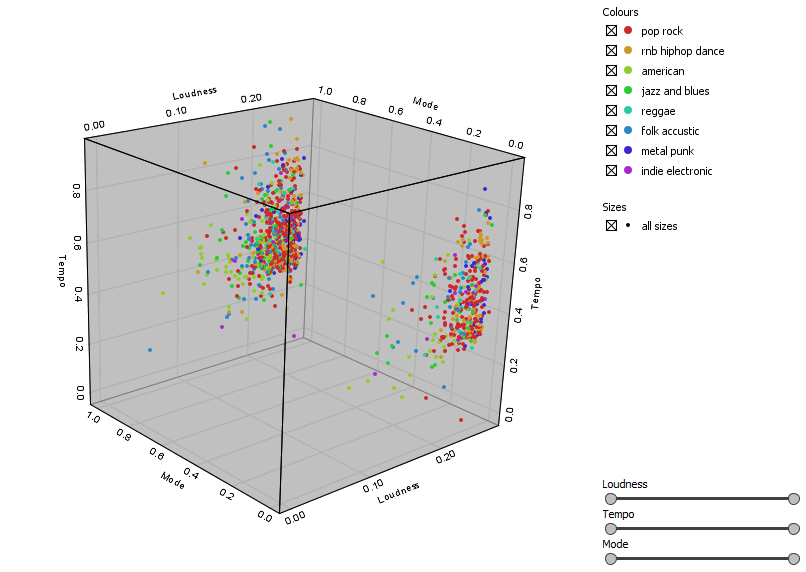
\includegraphics[scale=0.6]{resources/genre_scatter.PNG}
    \caption{3D prikaz pesama razli\v{c}itih \v{z}anrova u prostoru sa koordinatama \emph{loudness}, \emph{tempo} i \emph{mode}}
    \label{fig:ZanrKlasifikacija}
\end{figure}

\begin{figure}[H]
    \centering
    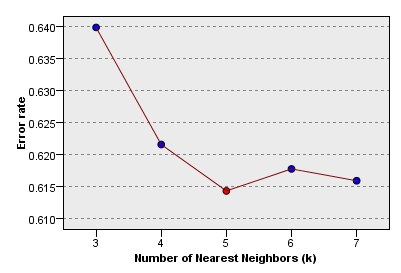
\includegraphics{resources/KNN_errors.PNG}
    \caption{Gre\v{s}ke dobijene za kreirane modele $k$ parametrom u opsegu $[3,7]$}
    \label{fig:KNNgreske}
\end{figure}

Ono \v{s}to nismo o\v{c}ekivali je jednaka va\v{z}nost atributa prilikom pravljenja klasifikatora - slika \ref{fig:KNNvaznost}. Intuicija nekako ka\v{z}e da su ja\v{c}e pesme podlo\v{z}nije da budu \v{z}anra \emph{metal}, ali rezultati su pobili tu intuiciju.

\begin{figure}[H]
    \centering
    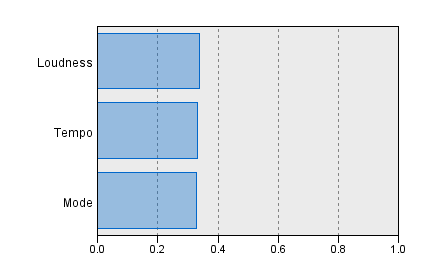
\includegraphics[scale=0.7]{resources/KNN_pred_imp.PNG}
    \caption{Va\v{z}nost atributa prilikom klasifikacije}
    \label{fig:KNNvaznost}
\end{figure}

Sled\'c{}i korak koji smo uradili bila je da isptobamo isti algoritam u alatu Knime \cite{KNIME} (prethodni zaklju\v{c}ci su dobijeni u alatu SPSS Modeler \cite{SPSS}). Ovo nam je pru\v{z}ilo mogu\'c{}nost da ru\v{c}no pridamo atributima ve\'c{}u ili manju va\v{z}nost. Iterativnim postupkom smo do\v{s}li do faktora kojima je potrebno pomno\v{z}iti vrednosti \emph{loudness} i \emph{tempo} kako bi se pove\'c{}ala preciznost klasifikatora. Ovo transformacija uti\v{c}e na izra\v{c}unavanje razli\v{c}itih euklidskih rastojanja izmedju pesama i dovela je do pobolj\v{s}anja preciznosti na $58.6\%$. Kori\v{s}\'c{}enje Menhetn rastojanja je dovelo do neznatno boljih rezultata, sa precizno\v{s}\'c{}u od $58.8\%$

Dodatno, jedno od mogu\'c{}ih unapredjenja bi bila da se u obzir uzme i atribut \emph{ModeConfidence}. Informacija o pouzdanosti vrednosti atributa koji predstavlja tonalitet pesme bi mogla da dovede do bolje klasifikacije.

\subsection{Klasifikacija stablom odlu\v{c}ivanja}
\label{subsec:stablo}
Predvidjanje \v{z}anra koriste\'c{}i stablo odlu\v{c}ivanja je takodje dalo lose rezultate. Preciznost dobijenog modela je $44.6\%$, te je gre\v{s}ka $55.4\%$. Matrica konfuzije je prikazana na slici \ref{fig:confmatrtree}.

\begin{center}
\begin{figure}[H]
    \centering
    \footnotesize
    \begin{tabular}{|c|c|c|c|c|c|c|c|c|}
        \hline
        & pop & hiphop & metal & & & jazz & accustic & indie \\
        Prediction & rock & rnb & punk & USA & reggae & blues & folk & electro \\
        & & dance & & & & & & \\
        \hline
        pop rock & 225 & 53 & 18 & 8 & 5 & 17 & 13 & 0 \\
        hiphop rnb dance & 48 & 10 & 11 & 0 & 1 & 3 & 1 & 0 \\
        metal punk & 32 & 11 & 7 & 0 & 0 & 0 & 1 & 0 \\
        american & 14 & 0 & 1 & 8 & 0 & 1 & 2 & 0 \\
        reggae & 7 & 2 & 0 & 0 & 0 & 1 & 3 & 0 \\
        jazz blues & 21 & 2 & 1 & 1 & 1 & 4 & 1 & 0 \\
        folk accustic & 18 & 4 & 2 & 1 & 1 & 3 & 2 & 0 \\
        indie electro & 6 & 1 & 0 & 1 & 0 & 0 & 0 & 0 \\
        \hline
    \end{tabular}
    \caption{Matrica konfuzije dobijena klasifikacijom stablom odlu\v{c}ivanja}
    \label{fig:confmatrtree}
\end{figure}
\end{center}

Na slici \ref{fig:tree} prikazano je dobijeno sablo odlu\v{c}ivanja. Kako vi\v{s}e od polovine pesama iz skupa pripada \v{z}anru \emph{pop rock}, a vrednosti atributa nisu dobre za klasifikaciju, stablo daje lo\v{s}e rezultate.


\begin{figure}[H]
    \centering
    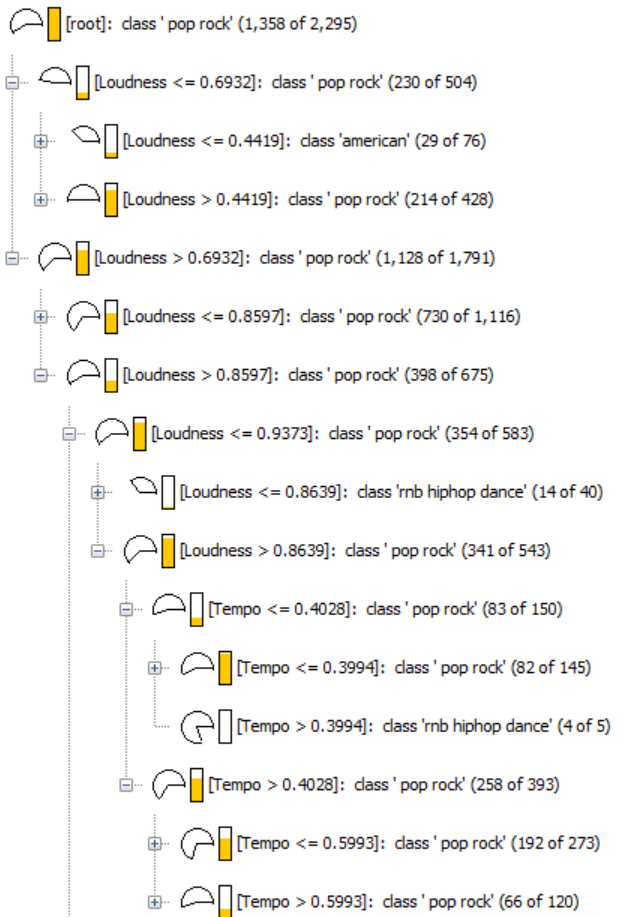
\includegraphics[scale=0.6]{resources/tree.png}
    \caption{Stablo odlu\v{c}ivanja za atrbut \v{z}anr}
    \label{fig:tree}
\end{figure}

\section{Zaključak}
\label{sec:Zakljucak}

Dobijeni rezultati se oslanjaju na podskup skupa podataka koji u sebi sadr\v{z}i milion pesama. Kori\v{s}\'c{}enje celog skupa podataka bi donelo jo\v{s} pouzdanije rezultate. Medjutim, i sam podskup podataka je bio dovoljan da se uo\v{c}e prethodno navedeni zaklju\v{c}ci.

Rezultati imaju prakti\v{c}nu primenu. Uo\v{c}avanje zavisnosti muzi\v{c}kih \v{z}anrova i godina njihove popularnosti, ili njihove popularnosti na razli\v{c}itim podnevljima bi se moglo iskoristiti za automatsko generisanje lista pesama. Ovo bi predstavljao zanimljiv i koristan dodatak za muzi\v{c}ki plejer.

Sajtovi kao \v{s}to su YouTube \cite{youtube} koriste prethodno prikupljene podatke o pesmama. Njih, u kombinaciji sa saznanjem o korisnikovim prethodno preslu\v{s}anim pesmama, koristi kako bi korisniku pru\v{z}io \v{s}to bolje preporuke za slede\'c{}u pesmu, a samim tim ga i zadr\v{z}ao na sajtu. Implementacija sli\v{c}nog, ali dosta jednostavnijeg, sistema bila bi mogu\'c{}a dobijenim rezultatima koji su predstavljeni u ovom radu.


\addcontentsline{toc}{section}{Literatura}
\bibliographystyle{plain}
\bibliography{literatura}

\newpage

\begin{appendices}
\section{Primer sloga}
\label{sec:DodatakPrimer}

\begin{figure}[H]
    \lstset{style=mystyle}
    \begin{lstlisting}[language=C, basicstyle=\footnotesize, numbers=none]
        analysis_sample_rate: 22050
        artist_7digitalid: 61424
        artist_familiarity: 0.5467275539627645
        artist_hotttnesss: 0.3861804160792181
        artist_id: ARE26EG1187B990AEF
        artist_latitude: 51.77045
        artist_location: Essex, England
        artist_longitude: 0.64255
        artist_mbid: de212b3a-2f54-4def-a13d-5a877bfaeaf7
        artist_mbtags: shape = (6,)
        artist_mbtags_count: shape = (6,)
        artist_name: Sunscreem
        artist_playmeid: 19156
        artist_terms: shape = (44,)
        artist_terms_freq: shape = (44,)
        artist_terms_weight: shape = (44,)
        audio_md5: c2f7f92e66d18e86af3752478d3be966
        bars_confidence: shape = (123,)
        bars_start: shape = (123,)
        beats_confidence: shape = (497,)
        beats_start: shape = (497,)
        danceability: 0.0
        duration: 232.4371
        end_of_fade_in: 0.0
        energy: 0.0
        key: 11
        key_confidence: 0.625
        loudness: -8.955
        mode: 0
        mode_confidence: 0.558
        release: Looking At You: The Club Anthems
        release_7digitalid: 196929
        sections_confidence: shape = (6,)
        sections_start: shape = (6,)
        segments_confidence: shape = (1045,)
        segments_loudness_max: shape = (1045,)
        segments_loudness_max_time: shape = (1045,)
        segments_loudness_start: shape = (1045,)
        segments_pitches: shape = (1045, 12)
        segments_start: shape = (1045,)
        segments_timbre: shape = (1045, 12)
        similar_artists: shape = (100,)
        song_hotttnesss: nan
        song_id: SOICLQB12A8C13637C
        start_of_fade_out: 232.437
        tatums_confidence: shape = (993,)
        tatums_start: shape = (993,)
        tempo: 130.201
        time_signature: 4
        time_signature_confidence: 0.0
        title: Exodus
        track_7digitalid: 2140010
        track_id: TRBBBLA128F424E963
        year: 1995
    \end{lstlisting}
    \caption{Primer sloga}
    \label{primer:Song}
\end{figure}

\section{Konverzija iz HDF5 u CSV format}
\label{sec:DodatakIzvlacenje}

\begin{figure}[H]
\lstset{style=mystyle}
\begin{lstlisting}[language=Python, basicstyle=\footnotesize]
"""
Alexis Greenstreet (October 4, 2015) University of Wisconsin-Madison
"""
class Song:
    songCount = 0

    def __init__(self, songID):
        self.id = songID
        Song.songCount += 1
        self.albumID = None                     # string
        self.albumName = None                   # string
        self.artistFamiliarity = None           # float
        self.artistHottnesss = None             # float
        self.artistID = None                    # string
        self.artistLatitude = None              # float
        self.artistLocation = None              # string
        self.artistLongitude = None             # float
        self.artistName = None                  # string
        self.audioMd5 = None                    # string
        self.danceability = None                # float
        self.duration = None                    # float
        self.endOfFadeIn = None                 # float
        self.energy = None                      # float
        self.genre = None                       # string
        self.genreList = []                     # list of strings
        self.key = None                         # int
        self.keyConfidence = None               # float
        self.keySignature = None                # float
        self.keySignatureConfidence = None      # float
        self.loudness = None                    # float
        self.mode = None                        # int
        self.modeConfidence = None              # float
        self.release = None                     # string
        self.songHotttness = None               # float
        self.songId = None                      # string
        self.startOfFadeOut = None              # float
        self.tempo = None                       # float
        self.timeSignature = None               # int
        self.timeSignatureConfidence = None     # float
        self.title = None                       # string
        self.trackId = None                     # string
        self.year = None                        # int
\end{lstlisting}
\label{code:SongClass}
\caption{Klasa kori\v{s}\'c{}ena za deserijalizaciju podataka.}
\end{figure}

\begin{figure}[H]
\lstset{style=mystyle}
\begin{lstlisting}[language=Python, basicstyle=\footnotesize]
"""
Alexis Greenstreet (October 4, 2015) University of Wisconsin-Madison
"""
outputFile1 = open('SongCSV.csv', 'w')
csvRowString = ""

csvRowString = ("SongID,AlbumID, ...")
	csvAttributeList = re.split('\W+', csvRowString)
for i, v in enumerate(csvAttributeList):
    csvAttributeList[i] = csvAttributeList[i].lower()
outputFile1.write("SongNumber,");
outputFile1.write(csvRowString + "\n");
csvRowString = ""

#################################################
#Set the basedir here, the root directory from which the search
basedir = "/home/m/Documents/MillionSongSubset/data"
ext = ".h5"
#################################################

csvRowStringTotal = ""

for root, dirs, files in os.walk(basedir):
    files = glob.glob(os.path.join(root,'*'+ext))
    for f in files:
        print f

        songH5File = hdf5_getters.open_h5_file_read(f)
        song = Song(str(hdf5_getters.get_song_id(songH5File)))

        song.artistID = str(hdf5_getters.get_artist_id(songH5File))
        # Isto za ostala polja

        artistMbtags = np.array(hdf5_getters.get_artist_mbtags(songH5File))
        song.genre = ' | '.join(artistMbtags)

        csvRowString += str(song.songCount) + ","
        csvRowString += song.id + ","
        # Isto za ostala polja

        csvRowString += song.trackId + ","
        csvRowString += song.genre + "\n"
        csvRowStringTotal += csvRowString
        csvRowString = ""

        songH5File.close()

outputFile1.write(csvRowStringTotal)
outputFile1.close()
\end{lstlisting}
\label{code:ConvertToCSV}
\caption{Upro\v{s}\'c{}ena verzija programa kori\v{s}\'c{}enog za konvertovanje iz HDF5 u CSV format.}
\end{figure}

\section{Statistika skupa podataka}
\label{sec:Statistika}

\begin{figure}[H]
\centering
\small
\Rotatebox{90}{%
    \begin{tabular}{|c|c|c|c|c|c|c|c|}
        \hline
        Column & ArtistLatitude & Duration & Loudness & Tempo & Year & Energy & Mode \\
        \hline
        Min & -41.281 & -114 & -51.643 & 0 & 1 & 0 & 0 \\
        Max & 151246 & 1815.222 & 261.538 & 262.828 & 2010 & 0.399 & 1 \\
        Mean & 94.001 & 238.379 & -10.444 & 122.868 & 1996.381 & 7.614E-05 & 0.691 \\
        Std. deviation & 2641.518 & 113.117 & 6.217 & 35.216 & 42.910 & 0.005 & 0.462 \\
        Variance & 6977616.187 & 12795.546 & 38.644 & 1240.182 & 1841.236 & 2.893E-05 & 0.21363 \\
        Skewness & 52.760 & 3.20372 & 8.711 & 0.404 & -43.0545 & 70.828 & -0.826 \\
        Kurtosis & 2922.508 & 24.813 & 396.106 & 0.487 & 1997.926 & 5029.175 & -1.319 \\
        Overall sum & 352221.307 & 2375926.299 & -104109.426 & 1224748.712 & 9317112 & 0.758 & 6876 \\
        No. missings & 6251 & 31 & 30 & 30 & 331 & 44 & 44 \\
        No. NaNs & 0 & 0 & 0 & 0 & 0 & 0 & 0 \\
        \hline
    \end{tabular}
}%
\caption{Statistike nama relevantnih atributa iz skupa}
\label{table:stats}
\end{figure}

\end{appendices}


\end{document}
